\documentclass[10pt]{article}
\usepackage{listings}
\usepackage[margin=1in]{geometry}
%Gummi|065|=)
\title{\textbf{EC450 Final Project | Team 8}}
\author{William Chen,
		Anton Paquin\\ \{chenwill, paquin\}@bu.edu}
\date{}
\usepackage{graphicx}
\usepackage{amsmath}
\usepackage{setspace}
\doublespacing

\begin{document}

\maketitle

\section{Goal and Design}

Our original project for this course involved emulating a GameCube controller for the purpose of performing tool-assisted superplay (TAS) routines on a GameCube or Wii game (for example, Super Smash Brothers Melee or Super Mario Sunshine). Unfortunately, we suffered a softbrick in one of the two MSP432 microprocessor boards at our disposal when attempting to set the main clock to its maximum speed (48MHz). Out of concern for breaking both boards and having no project as a result, we decided to abandon the aforementioned project and decided to venture into building a user-controllable miniature robot arm. \\ \newline
This robot arm was designed using five servo motors and had four joints; two drove a "shoulder" at the base, while three individual motors drove an elbow, wrist, and hand/claw. The MSP432 controlled actuation of these parts, and received commands from an internet-connected Raspberry Pi.

\section{Implementation}

From a system-level perspective, the three interacting hardware components involved the MSP432 microprocessor board, a robot arm built of five servo motors, and a Raspberry Pi 2. The MSP432 served as the interface that bridged user-defined inputs in software with the physical actuation of the robot arm. Hence, it connected to both the Raspberry Pi and the servo motors with the use of GPIO pins. \\ \newline
In terms of component-level peripherals used in the MSP432, we relied on the TimerA and the eUSCI SPI modules that drove the robot arm and communicated with the Raspberry Pi. 

\subsection{TimerA/Robot Arm}

Five TimerA configurations were set up and linked to each GPIO output connected to the servos, and the modules were run in capture compare mode to toggle a high and low signal when the half duty-cycle period was reached, creating a PWM signal that drive the servos to a fixed position. The duty cycle period is calculated in the servo\_set() function, which will set the appropriate compare value in the register (halfPeriod\--1) when given an input from 0\--180 (the range in degrees that the motors can move in).

\subsection{SPI/Raspberry Pi}

As the servo motors merely receive PWM signals and do not send any data in return, the communication link between the Raspberry Pi and the MSP432 only needed to be unidirectional, with data sent from the former into the latter. 
The SPI protocol was implemented between the two devices due to its simplicity. The Raspberry Pi was configured as the master, using a bitbanged software implementation written in Python. Meanwhile, using the eUSCI\_B SPI module with DriverLib code, the MSP432 was configured in a slave mode. Only three wires were actually needed (clock, MISO, and ground), as there was no need for slave select (only one device) or MOSI (no data from MSP432). \\ \newline
The command data sent from the Raspberry Pi to the MSP432 was a sequence of four bytes. Each byte corresponded to the degree that the joints should be set to (shoulder, elbow, wrist, and hand, respectively), and therefore were values from 0x00 to 0xB4 (0\--180). Since two servos in the shoulder controlled the same joint, we were able to use one less byte by having the MSP432 calculate the degree of the second servo as 180\--x. On the MSP432, an array of four chars was created as a command buffer, and a byte was added during each eUSCI RX interrupt as part of the handler. When the array was full (as determined by an incrementing counter), the eUSCI interrupt handler called servo\_set() to set the appropriate PWM signals that moved the servos to the degrees specified in the array, emptied the buffer, and reset the counter. \\ \newline
From the Raspberry Pi, it was very simple to pass a list of four ints (from 0 to 180) into a loop that calls the SPI write function for each byte. Given the flexibility of Python and a small portable Linux computer in the Raspberry Pi, it was easy to set up a simple GUI that can be internet-connected (just for fun).





\section{Schematic}

\begin{figure}[htp]
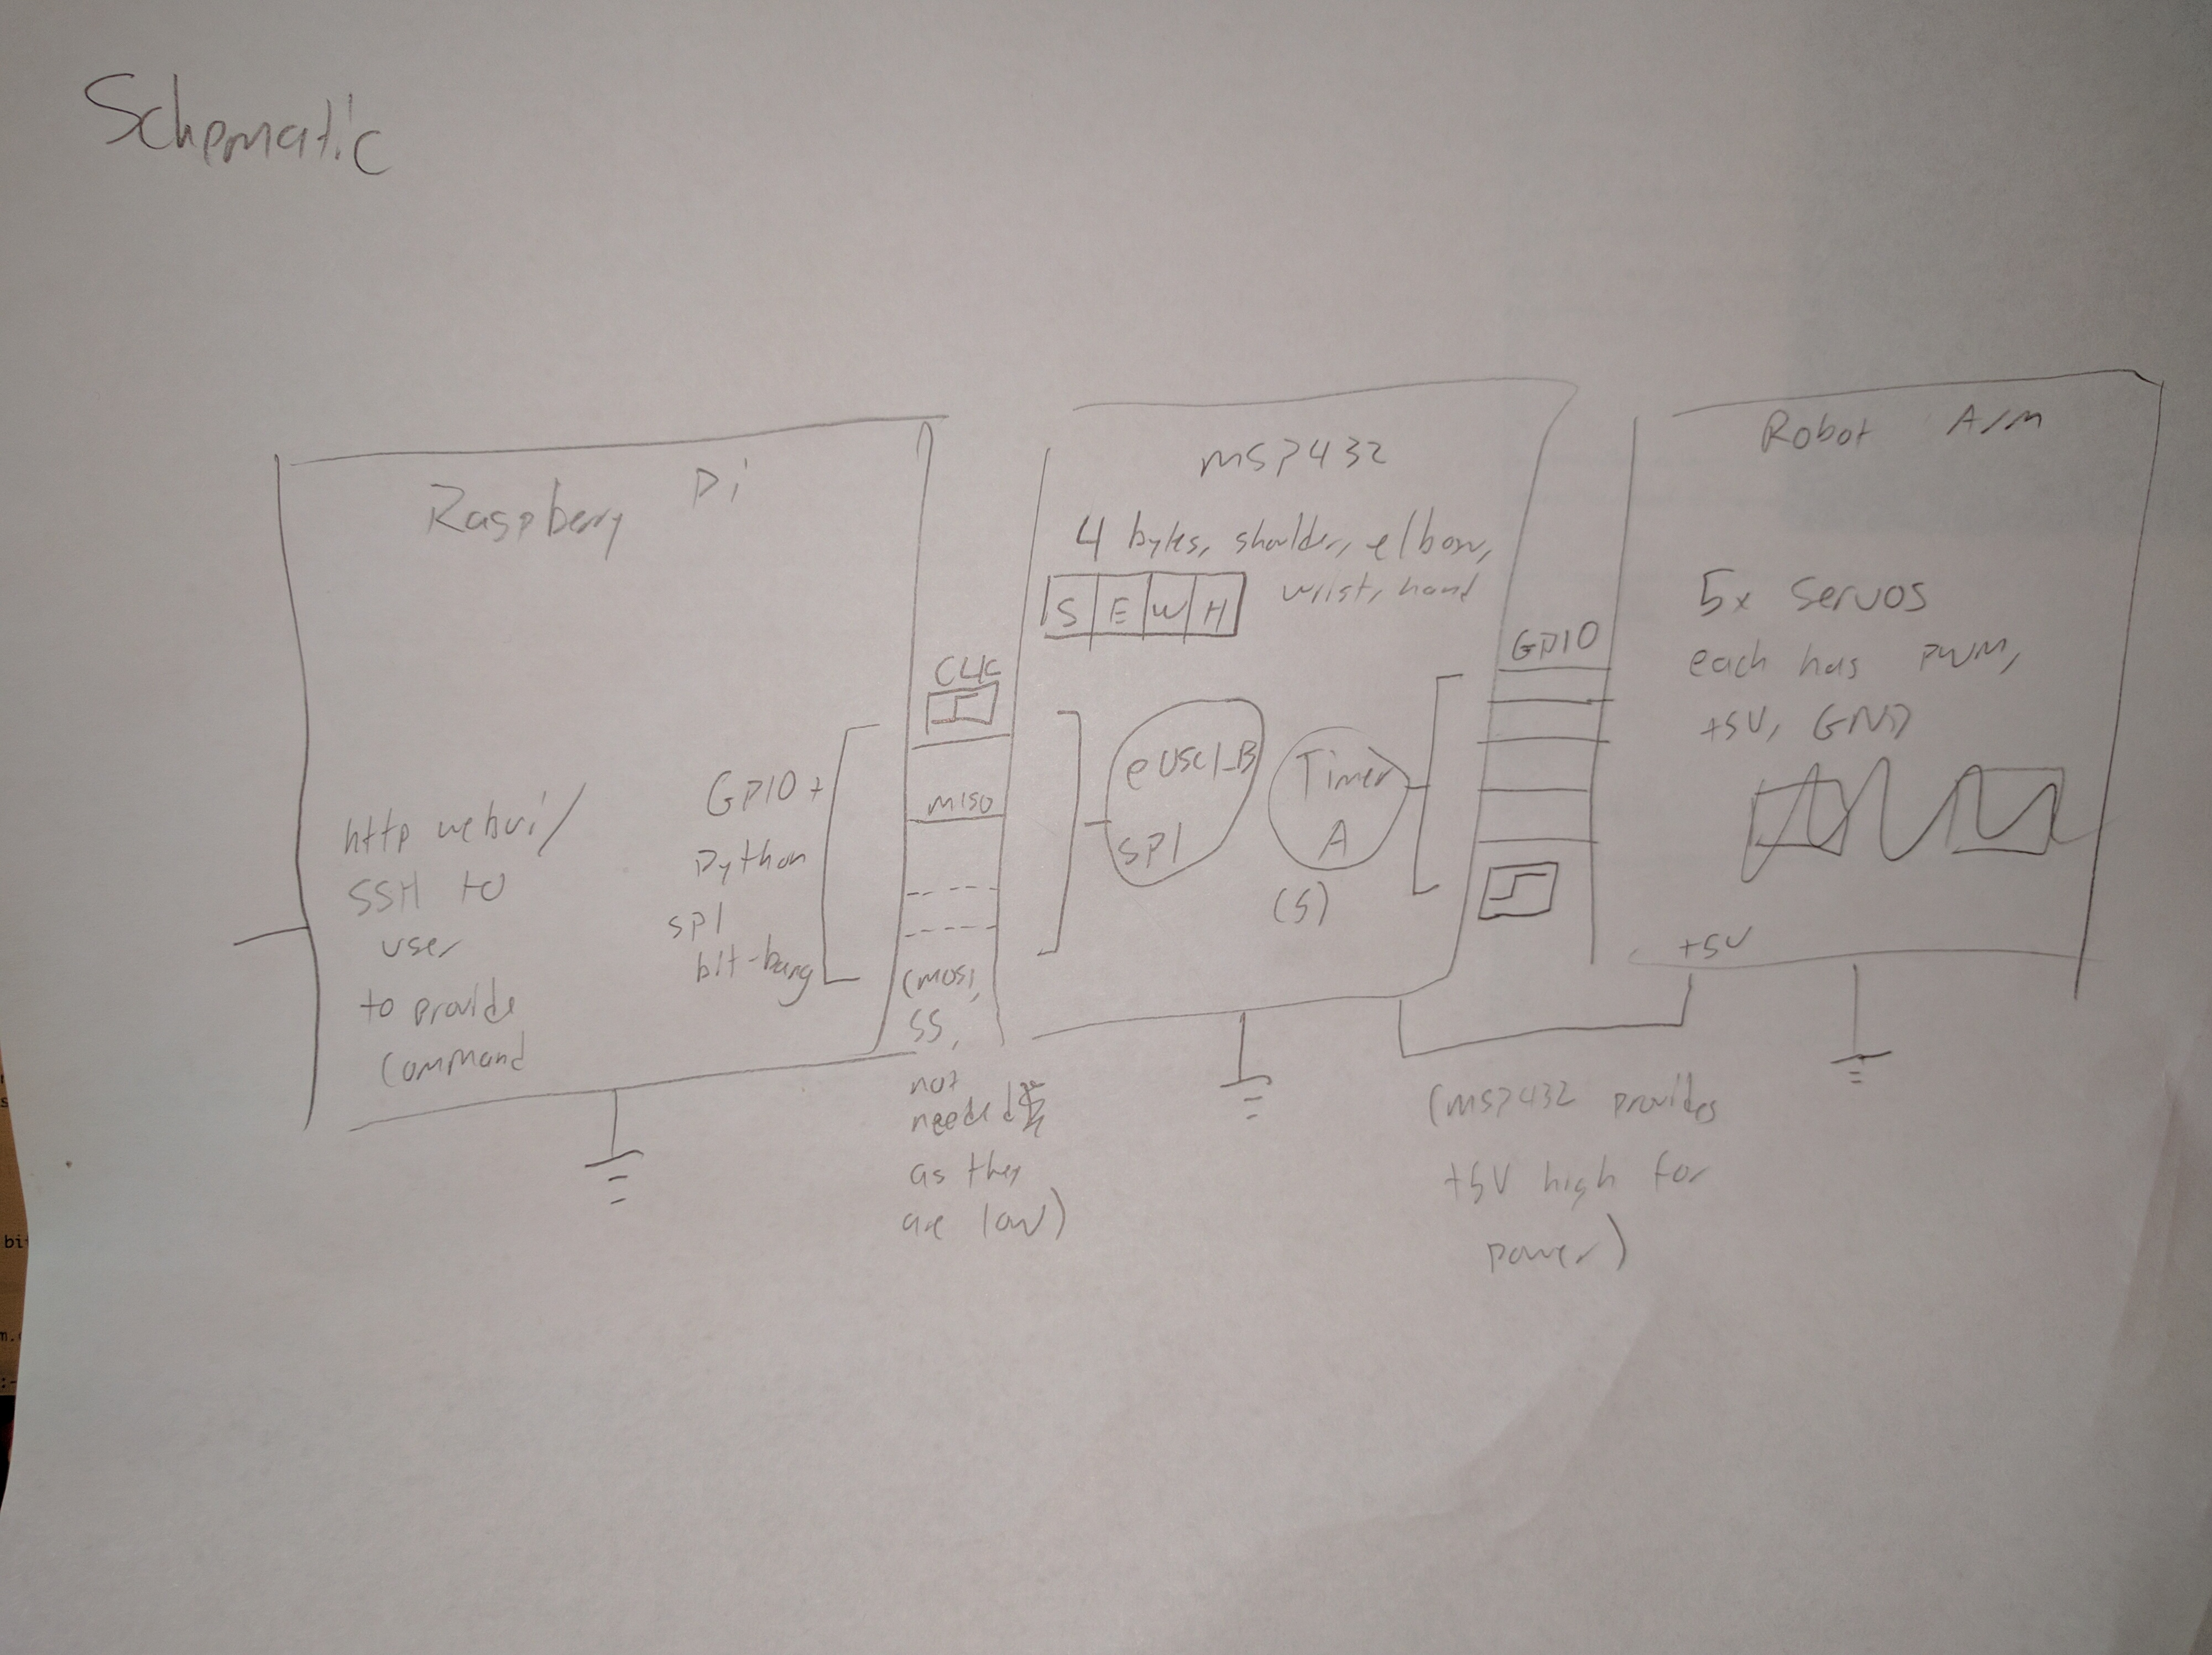
\includegraphics[width=\linewidth]{IMG_20170507_211043}
\caption{Block-level diagram}
\end{figure}


\section{Outcome}

The robot arm responded to inputs fairly accurately in terms of the specified degree requested compared to the actual measured value. The four bytes that were sent were received correctly, however, it was not always perfect. Of note, the MSP432 eUSCI SPI implementation sometimes did appear to exhibit some transfer errors. For example, values may have been bit shifted and some bytes were occasionally dropped, causing the elbow to be actuated instead of the shoulder or an incorrect degree value would be inserted. Improvements to the mechanical and communications systems are suggested as follows.

\section{Improvements}
While the servos were fairly accurate when calibrated, they were quite cheap and susceptible to heat problems and audible noise, potentially making them unsafe for long-term use. \\ \newline
From the communications perspective, some control bytes and/or parity bits could be added to the protocol ensuring that the commands are always correct.
\section{Code}


All the code can be found on GitHub at 
\begin{lstlisting}
https://github.com/antonpaquin/EC450-proj
\end{lstlisting}
For the sake of convenience, the library routines and main.c are provided in the archive containing this report.

\section{Human Resources}
Anton was responsible for writing code involved with driving the individual servo motors as a library routine and debugged the finished product (calibration values).\\ \newline 
Will was responsible for the communications interface between the MSP432 and the Raspberry Pi (SPI).





%\begin{figure}[htp]
%\centering
%\includegraphics[scale=0.25]{"/home/anton/Documents/School/BU 2017 Spring/EC506/Proj/discover-shot".png}
%\caption{Go see these at http://eftychis.antonpaqu.in:5601}
%\label{}
%\end{figure}

\end{document}
